\chapter{Syklittömät verkot}

Keskeinen hankaluus verkkoalgoritmien suunnittelussa ovat
verkossa olevat syklit.
Jos voidaan olettaa, että verkossa ei ole syklejä,
monen ongelman ratkaisu onkin paljon helpompaa.
Silloin verkon voi jakaa luontevasti pienempiin osiin,
joihin voi soveltaa esimerkiksi dynaamista ohjelmointia.

Tässä luvussa tutustumme algoritmeihin,
jotka käsittelevät suunnattuja, syklittömiä verkkoja.
Tämä verkkotyypi on niin tärkeä, että englannin kielessä
on sille oma lyhenne \textit{dag},
joka tulee sanoista \textit{directed acyclic graph}.

\section{Syklin etsiminen}

Miten voi tietää, onko suunnatussa verkossa
sykliä?
Yksi tehokas menetelmä on etsiä
sykliä käyttäen muunnettua syvyyshakua.

Ideana on toteuttaa syvyyshaku niin,
että solmulla on kolme mahdollista tilaa:
0 (ei käsitelty),
1 (käsittely kesken) tai
2 (käsittely valmis).
Aluksi jokaisen solmun tilana on 0.
Tila 1 aktivoituu,
kun haku tulee solmuun ensimmäistä kertaa,
ja tilaksi tulee 2,
kun kaikki solmusta lähtevät kaaret
on käsitelty.

Verkossa on suunnattu sykli tarkalleen silloin,
jos jossain vaiheessa syvyyshakua vastaan
tulee tilassa 1 oleva solmu.
Sykli muodostuu niistä solmuista,
joihin haku on edennyt tilassa 1
olevan solmun jälkeen.

Tässä on algoritmin toteutus:

\begin{lstlisting}
void haku(int s) {
    if (t[s] == 1) {
        // suunnattu sykli löytyi
        return;
    }
    if (t[s] == 2) return;
    t[s] = 1;
    for (int i = 0; i < v[s].size(); i++) {
        haku(v[s][i]);
    }
    t[s] = 2;
}
\end{lstlisting}

\section{Topologinen järjestys}

Suunnatun verkon topologinen järjestys
(\textit{topological sort}) on
sellainen lista solmuista,
että jos solmusta $a$ on kaari solmuun $b$,
niin $a$ on ennen $b$:tä listassa.
Esimerkiksi jos solmut ovat kursseja
ja kaaret kuvaavat kurssien esitietovaatimukset,
topologinen järjestys antaa yhden
tavan suorittaa kaikki kurssit.

Esimerkiksi verkon
\begin{center}
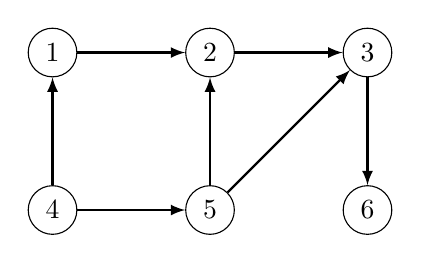
\begin{tikzpicture}
\node[draw, circle] (1) at (1,5) {$1$};
\node[draw, circle] (2) at (3,5) {$2$};
\node[draw, circle] (3) at (5,5) {$3$};
\node[draw, circle] (4) at (1,3) {$4$};
\node[draw, circle] (5) at (3,3) {$5$};
\node[draw, circle] (6) at (5,3) {$6$};

\path[draw,thick,->,>=latex] (1) -- (2);
\path[draw,thick,->,>=latex] (2) -- (3);
\path[draw,thick,->,>=latex] (4) -- (1);
\path[draw,thick,->,>=latex] (4) -- (5);
\path[draw,thick,->,>=latex] (5) -- (2);
\path[draw,thick,->,>=latex] (5) -- (3);
\path[draw,thick,->,>=latex] (3) -- (6);
\end{tikzpicture}
\end{center}

yksi topologinen järjestys on
4, 1, 5, 2, 3, 6:
\begin{center}
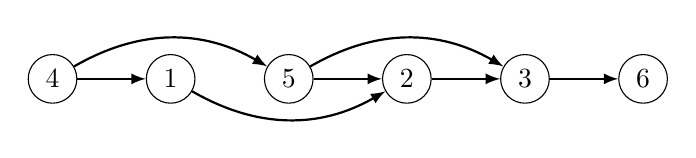
\begin{tikzpicture}
\node[draw, circle] (1) at (-6,0) {$1$};
\node[draw, circle] (2) at (-3,0) {$2$};
\node[draw, circle] (3) at (-1.5,0) {$3$};
\node[draw, circle] (4) at (-7.5,0) {$4$};
\node[draw, circle] (5) at (-4.5,0) {$5$};
\node[draw, circle] (6) at (-0,0) {$6$};

\path[draw,thick,->,>=latex] (1) edge [bend right=30] (2);
\path[draw,thick,->,>=latex] (2) -- (3);
\path[draw,thick,->,>=latex] (4) -- (1);
\path[draw,thick,->,>=latex] (4) edge [bend left=30] (5);
\path[draw,thick,->,>=latex] (5) -- (2);
\path[draw,thick,->,>=latex] (5) edge [bend left=30]  (3);
\path[draw,thick,->,>=latex] (3) -- (6);
\end{tikzpicture}
\end{center}


Topologinen järjestys on olemassa
silloin, kun verkossa ei ole suunnattua sykliä.
Jos verkossa on suunnattu sykli,
topologista järjestystä ei voi muodostaa,
koska mitään syklin solmuista
ei voi valita järjestykseen ensimmäisenä.

Kätevä tapa muodostaa topologinen järjestys
on valita järjestykseen aina
seuraavaksi sellainen solmu, johon ei tule kaaria muista solmuista.
Jos mahdollisia solmuja on useita,
niistä voi valita minkä tahansa.
Sitten valittu solmu ja
siitä lähtevät kaaret poistetaan verkosta.
Sama jatkuu niin kauan,
kunnes kaikki solmut on valittu ja topologinen
järjestys on valmis.

Esimerkkiverkossa ensimmäinen valittava
solmu on 4:
\begin{center}
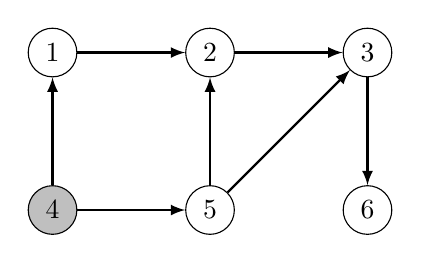
\begin{tikzpicture}
\node[draw, circle] (1) at (1,5) {$1$};
\node[draw, circle] (2) at (3,5) {$2$};
\node[draw, circle] (3) at (5,5) {$3$};
\node[draw, circle, fill=lightgray] (4) at (1,3) {$4$};
\node[draw, circle] (5) at (3,3) {$5$};
\node[draw, circle] (6) at (5,3) {$6$};

\path[draw,thick,->,>=latex] (1) -- (2);
\path[draw,thick,->,>=latex] (2) -- (3);
\path[draw,thick,->,>=latex] (4) -- (1);
\path[draw,thick,->,>=latex] (4) -- (5);
\path[draw,thick,->,>=latex] (5) -- (2);
\path[draw,thick,->,>=latex] (5) -- (3);
\path[draw,thick,->,>=latex] (3) -- (6);
\end{tikzpicture}
\end{center}
Solmun poistamisen jälkeen solmuihin
1 ja 5 ei tule kaaria, joten jompikumpi
niistä valitaan seuraavaksi topologiseen järjestykseen:
\begin{center}
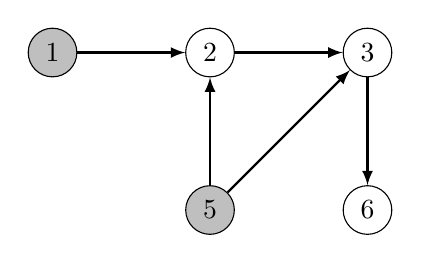
\begin{tikzpicture}
\node[draw, circle, fill=lightgray] (1) at (1,5) {$1$};
\node[draw, circle] (2) at (3,5) {$2$};
\node[draw, circle] (3) at (5,5) {$3$};
%\node[draw, circle, fill=lightgray] (4) at (1,3) {$4$};
\node[draw, circle, fill=lightgray] (5) at (3,3) {$5$};
\node[draw, circle] (6) at (5,3) {$6$};

\path[draw,thick,->,>=latex] (1) -- (2);
\path[draw,thick,->,>=latex] (2) -- (3);
%\path[draw,thick,->,>=latex] (4) -- (1);
%\path[draw,thick,->,>=latex] (4) -- (5);
\path[draw,thick,->,>=latex] (5) -- (2);
\path[draw,thick,->,>=latex] (5) -- (3);
\path[draw,thick,->,>=latex] (3) -- (6);
\end{tikzpicture}
\end{center}

Solmujen valinta jatkuu vastaavasti, kunnes
topologinen järjestys on valmis.
Verkon syklittömyys takaa, että jokin solmu
on aina mahdollista valita,
koska jos kaikkiin solmuihin tulisi
kaari toisesta solmusta, niin verkossa olisi sykli.

\section{Dynaaminen ohjelmointi}

Syklittömässä verkossa topologinen järjestys
antaa luontevan tavan käsitellä solmut
niiden riippuvuuksien mukaisessa järjestyksessä.
Tämän ansiosta verkon käsittelyssä voi käyttää
dynaamista ohjelmointia niin, että jokaiseen solmuun
lasketaan haluttu asia siihen tulevien kaarten perusteella.

\subsection{Pisin polku}

\begin{task}
Annettuna on suunnattu, syklitön verkko,
ja tehtäväsi on etsiä verkosta \textit{pisin}
polku, joka kulkee solmusta $a$ solmuun $b$.
\end{task}

Esimerkiksi verkossa 
\begin{center}
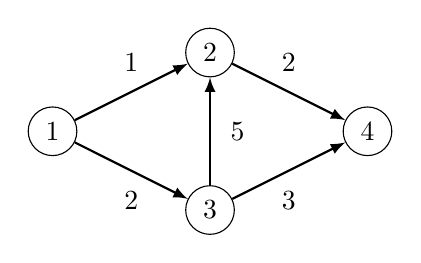
\begin{tikzpicture}
\node[draw, circle] (1) at (0,0) {$1$};
\node[draw, circle] (2) at (2,1) {$2$};
\node[draw, circle] (3) at (2,-1) {$3$};
\node[draw, circle] (4) at (4,0) {$4$};

\path[draw,thick,->,>=latex] (1) -- node[font=\small,label=above:1] {} (2);
\path[draw,thick,->,>=latex] (1) -- node[font=\small,label=below:2] {} (3);
\path[draw,thick,->,>=latex] (3) -- node[font=\small,label=right:5] {} (2);
\path[draw,thick,->,>=latex] (2) -- node[font=\small,label=above:2] {} (4);
\path[draw,thick,->,>=latex] (3) -- node[font=\small,label=below:3] {} (4);
\end{tikzpicture}
\end{center}
pisin polku solmusta 1 solmuun 4
kulkee kaaria $1 \rightarrow 3 \rightarrow 2 \rightarrow 2$
ja sen pituus on $2+5+2=9$.

Yleisessä verkossa pisimmän polun etsiminen
on NP-vaikea ongelma, eikä siihen tunneta
mitään tehokasta algoritmia.
Syklittömässä verkossa tehtävä on kuitenkin
mahdollista ratkaista tehokkaasti
dynaamisella ohjelmoinnilla.

Ideana on laskea
jokaiseen solmuun $s$, kuinka pitkä on pisin
polku alkusolmusta solmuun $s$.
Jos solmu $s$ on alkusolmu,
pisimmän polun pituus on 0.
Muuten polun pituuden saa laskettua
käymällä läpi solmuun tulevat
kaaret ja valitsemalla
pisimmän polun tuottava kaari.

Esimerkkiverkossa laskenta lähtee liikkeelle
siitä, että pisin solmuun 1 johtava
polku on pituudeltaan 0:

\begin{center}
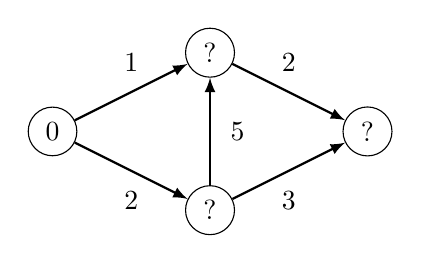
\begin{tikzpicture}
\node[draw, circle] (1) at (0,0) {$0$};
\node[draw, circle] (2) at (2,1) {?};
\node[draw, circle] (3) at (2,-1) {?};
\node[draw, circle] (4) at (4,0) {?};

\path[draw,thick,->,>=latex] (1) -- node[font=\small,label=above:1] {} (2);
\path[draw,thick,->,>=latex] (1) -- node[font=\small,label=below:2] {} (3);
\path[draw,thick,->,>=latex] (3) -- node[font=\small,label=right:5] {} (2);
\path[draw,thick,->,>=latex] (2) -- node[font=\small,label=above:2] {} (4);
\path[draw,thick,->,>=latex] (3) -- node[font=\small,label=below:3] {} (4);
\end{tikzpicture}
\end{center}

Seuraavana topologisessa järjestyksessä on solmu 3,
johon johtavan pisimmän polun pituus on 2,
koska sinne voi tulla vain solmusta 1:

\begin{center}
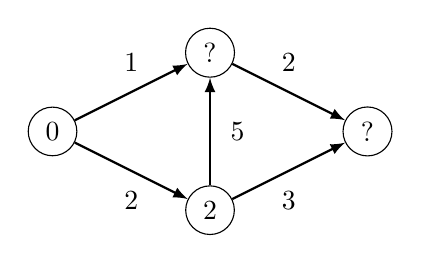
\begin{tikzpicture}
\node[draw, circle] (1) at (0,0) {$0$};
\node[draw, circle] (2) at (2,1) {?};
\node[draw, circle] (3) at (2,-1) {$2$};
\node[draw, circle] (4) at (4,0) {?};

\path[draw,thick,->,>=latex] (1) -- node[font=\small,label=above:1] {} (2);
\path[draw,thick,->,>=latex] (1) -- node[font=\small,label=below:2] {} (3);
\path[draw,thick,->,>=latex] (3) -- node[font=\small,label=right:5] {} (2);
\path[draw,thick,->,>=latex] (2) -- node[font=\small,label=above:2] {} (4);
\path[draw,thick,->,>=latex] (3) -- node[font=\small,label=below:3] {} (4);
\end{tikzpicture}
\end{center}

Solmuun 2 voi tulla sekä solmusta 1 että solmusta 3,
ja pisin reitti pituudella 7 syntyy tulemalla solmusta 3:

\begin{center}
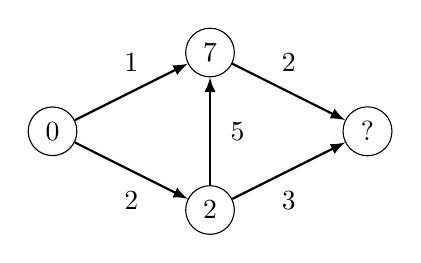
\begin{tikzpicture}
\node[draw, circle] (1) at (0,0) {$0$};
\node[draw, circle] (2) at (2,1) {$7$};
\node[draw, circle] (3) at (2,-1) {$2$};
\node[draw, circle] (4) at (4,0) {?};

\path[draw,thick,->,>=latex] (1) -- node[font=\small,label=above:1] {} (2);
\path[draw,thick,->,>=latex] (1) -- node[font=\small,label=below:2] {} (3);
\path[draw,thick,->,>=latex] (3) -- node[font=\small,label=right:5] {} (2);
\path[draw,thick,->,>=latex] (2) -- node[font=\small,label=above:2] {} (4);
\path[draw,thick,->,>=latex] (3) -- node[font=\small,label=below:3] {} (4);
\end{tikzpicture}
\end{center}

Lopulta saadaan laskettua pisin reitti solmuun 4:
\begin{center}
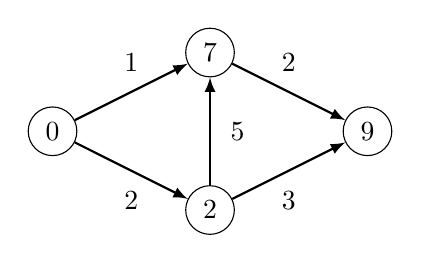
\begin{tikzpicture}
\node[draw, circle] (1) at (0,0) {$0$};
\node[draw, circle] (2) at (2,1) {$7$};
\node[draw, circle] (3) at (2,-1) {$2$};
\node[draw, circle] (4) at (4,0) {$9$};

\path[draw,thick,->,>=latex] (1) -- node[font=\small,label=above:1] {} (2);
\path[draw,thick,->,>=latex] (1) -- node[font=\small,label=below:2] {} (3);
\path[draw,thick,->,>=latex] (3) -- node[font=\small,label=right:5] {} (2);
\path[draw,thick,->,>=latex] (2) -- node[font=\small,label=above:2] {} (4);
\path[draw,thick,->,>=latex] (3) -- node[font=\small,label=below:3] {} (4);
\end{tikzpicture}
\end{center}

\subsection{Polkujen määrä}

\begin{task}
Annettuna on suunnattu, syklitön verkko,
ja tehtäväsi on laskea,
montako polkua verkossa on solmusta $a$ solmuun $b$.
\end{task}

Esimerkiksi verkossa 
\begin{center}
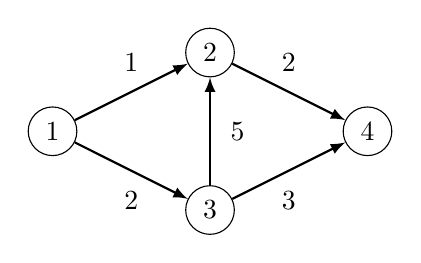
\begin{tikzpicture}
\node[draw, circle] (1) at (0,0) {$1$};
\node[draw, circle] (2) at (2,1) {$2$};
\node[draw, circle] (3) at (2,-1) {$3$};
\node[draw, circle] (4) at (4,0) {$4$};

\path[draw,thick,->,>=latex] (1) -- node[font=\small,label=above:1] {} (2);
\path[draw,thick,->,>=latex] (1) -- node[font=\small,label=below:2] {} (3);
\path[draw,thick,->,>=latex] (3) -- node[font=\small,label=right:5] {} (2);
\path[draw,thick,->,>=latex] (2) -- node[font=\small,label=above:2] {} (4);
\path[draw,thick,->,>=latex] (3) -- node[font=\small,label=below:3] {} (4);
\end{tikzpicture}
\end{center}
solmusta 1 solmuun 4 on 3 mahdollista polkua:
\begin{itemize}
\item $1 \rightarrow 2 \rightarrow 4$
\item $1 \rightarrow 3 \rightarrow 2 \rightarrow 4$
\item $1 \rightarrow 3 \rightarrow 4$
\end{itemize}
Polkujen määrän saa laskettua dynaamisella
ohjelmoinnilla lähes samalla tavalla
kuin pisimmän polun pituuden.
Ainoa ero on, että jokaiseen solmuun lasketaan
siihen johtavien polkujen määrä:
\begin{center}
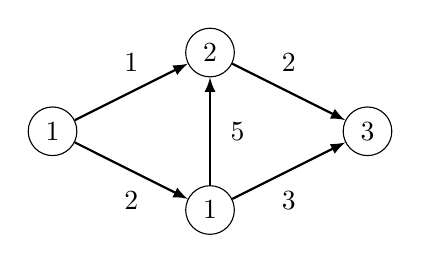
\begin{tikzpicture}
\node[draw, circle] (1) at (0,0) {$1$};
\node[draw, circle] (2) at (2,1) {$2$};
\node[draw, circle] (3) at (2,-1) {$1$};
\node[draw, circle] (4) at (4,0) {$3$};

\path[draw,thick,->,>=latex] (1) -- node[font=\small,label=above:1] {} (2);
\path[draw,thick,->,>=latex] (1) -- node[font=\small,label=below:2] {} (3);
\path[draw,thick,->,>=latex] (3) -- node[font=\small,label=right:5] {} (2);
\path[draw,thick,->,>=latex] (2) -- node[font=\small,label=above:2] {} (4);
\path[draw,thick,->,>=latex] (3) -- node[font=\small,label=below:3] {} (4);
\end{tikzpicture}
\end{center}

\subsection{Tulkinta verkkona}

Itse asiassa dynaamista ohjelmointia voi
ajatella \textit{aina} suunnatun,
syklittömän verkon käsittelynä.
Verkon solmut ovat dynaamisen ohjelmoinnin
tilat ja kaaret kuvaavat, miten tilat
riippuvat toisistaan.

Tarkastellaan esimerkiksi seuraavaa
tuttua tehtävää:

\begin{task}
Kolikoiden arvot ovat $\{c_1,c_2,\ldots,c_k\}$,
ja tehtäväsi on muodostaa kolikoista rahamäärä $x$.
Jokaista kolikkoa on saatavilla rajattomasti.
Mikä on pienin määrä kolikoita,
joilla rahamäärän voi muodostaa?
\end{task}

Ideana on luoda verkko,
jossa solmut vastaavat mahdollisia rahamääriä
ja kaaret kuvaavat tapoja viedä ratkaisua
eteenpäin käyttäen saatavilla olevia kolikoita.
Esimerkiksi jos kolikot ovat $\{1,3,4\}$
ja rahamäärä on 6, verkosta tulee seuraavanlainen:
\begin{center}
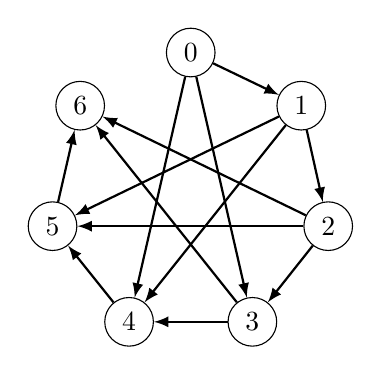
\begin{tikzpicture}[scale=0.9]
\node[draw, circle] (0) at (0,2) {$0$};
\node[draw, circle] (1) at (1.56,1.25) {$1$};
\node[draw, circle] (2) at (1.94,-0.45) {$2$};
\node[draw, circle] (3) at (0.87,-1.80) {$3$};
\node[draw, circle] (4) at (-0.87,-1.80) {$4$};
\node[draw, circle] (5) at (-1.95,-0.45) {$5$};
\node[draw, circle] (6) at (-1.56,1.25) {$6$};

\path[draw,thick,<-,>=latex] (1) -- (0);
\path[draw,thick,<-,>=latex] (2) -- (1);
\path[draw,thick,<-,>=latex] (3) -- (2);
\path[draw,thick,<-,>=latex] (4) -- (3);
\path[draw,thick,<-,>=latex] (5) -- (4);
\path[draw,thick,<-,>=latex] (6) -- (5);

\path[draw,thick,<-,>=latex] (3) -- (0);
\path[draw,thick,<-,>=latex] (4) -- (1);
\path[draw,thick,<-,>=latex] (5) -- (2);
\path[draw,thick,<-,>=latex] (6) -- (3);

\path[draw,thick,<-,>=latex] (4) -- (0);
\path[draw,thick,<-,>=latex] (5) -- (1);
\path[draw,thick,<-,>=latex] (6) -- (2);
\end{tikzpicture}
\end{center}
Optimiratkaisua $3+3=6$ vastaa seuraava kaarten valinta:
\begin{center}
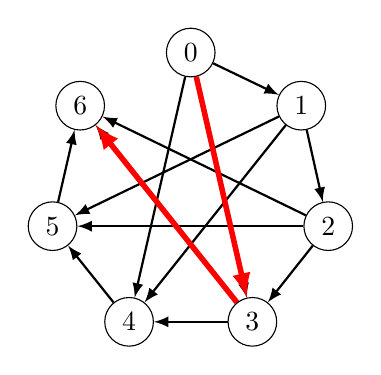
\begin{tikzpicture}[scale=0.9]
\node[draw, circle] (0) at (0,2) {$0$};
\node[draw, circle] (1) at (1.56,1.25) {$1$};
\node[draw, circle] (2) at (1.94,-0.45) {$2$};
\node[draw, circle] (3) at (0.87,-1.80) {$3$};
\node[draw, circle] (4) at (-0.87,-1.80) {$4$};
\node[draw, circle] (5) at (-1.95,-0.45) {$5$};
\node[draw, circle] (6) at (-1.56,1.25) {$6$};

\path[draw,thick,<-,>=latex] (1) -- (0);
\path[draw,thick,<-,>=latex] (2) -- (1);
\path[draw,thick,<-,>=latex] (3) -- (2);
\path[draw,thick,<-,>=latex] (4) -- (3);
\path[draw,thick,<-,>=latex] (5) -- (4);
\path[draw,thick,<-,>=latex] (6) -- (5);

\path[draw,thick,<-,>=latex] (3) -- (0);
\path[draw,thick,<-,>=latex] (4) -- (1);
\path[draw,thick,<-,>=latex] (5) -- (2);
\path[draw,thick,<-,>=latex] (6) -- (3);

\path[draw,thick,<-,>=latex] (4) -- (0);
\path[draw,thick,<-,>=latex] (5) -- (1);
\path[draw,thick,<-,>=latex] (6) -- (2);

\path[draw,thick,->,>=latex,red,line width=2pt] (0) -- (3);
\path[draw,thick,->,>=latex,red,line width=2pt] (3) -- (6);
\end{tikzpicture}
\end{center}

\section{Dijkstran muunnelmat}

Dijkstran algoritmin tuloksena on suunnattu,
syklitön verkko, joka kertoo,
mitkä verkon kaaret kuuluvat johonkin
lyhimpään polkuun alkusolmusta lähtien.
Esimerkiksi verkossa
\begin{center}
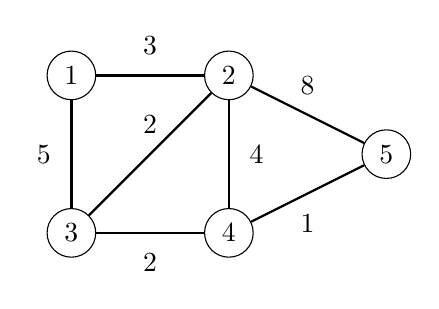
\begin{tikzpicture}
\node[draw, circle] (1) at (0,0) {$1$};
\node[draw, circle] (2) at (2,0) {$2$};
\node[draw, circle] (3) at (0,-2) {$3$};
\node[draw, circle] (4) at (2,-2) {$4$};
\node[draw, circle] (5) at (4,-1) {$5$};

\path[draw,thick,-] (1) -- node[font=\small,label=above:3] {} (2);
\path[draw,thick,-] (1) -- node[font=\small,label=left:5] {} (3);
\path[draw,thick,-] (2) -- node[font=\small,label=right:4] {} (4);
\path[draw,thick,-] (2) -- node[font=\small,label=above:8] {} (5);
\path[draw,thick,-] (3) -- node[font=\small,label=below:2] {} (4);
\path[draw,thick,-] (4) -- node[font=\small,label=below:1] {} (5);
\path[draw,thick,-] (2) -- node[font=\small,label=above:2] {} (3);
\end{tikzpicture}
\end{center}

solmusta 1 lähteviin lyhimpiin polkuihin kuuluvat
seuraavat kaaret:
\begin{center}
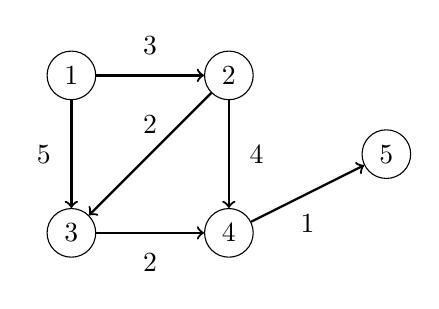
\begin{tikzpicture}
\node[draw, circle] (1) at (0,0) {$1$};
\node[draw, circle] (2) at (2,0) {$2$};
\node[draw, circle] (3) at (0,-2) {$3$};
\node[draw, circle] (4) at (2,-2) {$4$};
\node[draw, circle] (5) at (4,-1) {$5$};

\path[draw,thick,->] (1) -- node[font=\small,label=above:3] {} (2);
\path[draw,thick,->] (1) -- node[font=\small,label=left:5] {} (3);
\path[draw,thick,->] (2) -- node[font=\small,label=right:4] {} (4);
\path[draw,thick,->] (3) -- node[font=\small,label=below:2] {} (4);
\path[draw,thick,->] (4) -- node[font=\small,label=below:1] {} (5);
\path[draw,thick,->] (2) -- node[font=\small,label=above:2] {} (3);
\end{tikzpicture}
\end{center}
Koska kyseessä on suunnaton, syklitön verkko,
siihen voi soveltaa dynaamista ohjelmointia.
Näin saadaan vastaukset esimerkiksi seuraaviin kysymyksiin:

\begin{itemize}
\item montako erilaista lyhintä polkua on solmusta $a$ solmuun $b$?
\item mikä on pienin ja suurin mahdollinen kaarten määrä lyhimmällä polulla?
\item mitkä solmut esiintyvät varmasti lyhimmällä polulla?
\end{itemize}

Esimerkiksi yllä olevassa verkossa
solmusta 1 solmuun 5 on 3 erilaista lyhintä polkua,
pienin kaarten määrä on 3,
suurin kaarten määrä on 4, ja
solmut 1, 4 ja 5 esiintyvät varmasti lyhimmällä polulla.